% 
% ---------------------------------------------------------------
% Copyright (C) 2012-2018 Gang Li
% ---------------------------------------------------------------
%
% This work is the default powerdot-tuliplab style test file and may be
% distributed and/or modified under the conditions of the LaTeX Project Public
% License, either version 1.3 of this license or (at your option) any later
% version. The latest version of this license is in
% http://www.latex-project.org/lppl.txt and version 1.3 or later is part of all
% distributions of LaTeX version 2003/12/01 or later.
%
% This work has the LPPL maintenance status "maintained".
%
% This Current Maintainer of this work is Gang Li.
%
%

\documentclass[
 size=12pt,
 paper=smartboard, %a4paper, smartboard, screen
 mode=present, %present, handout, print
 display=slides, % slidesnotes, notes, slides
% nohandoutpagebreaks,
% pauseslide,
style=tuliplab,
% nopagebreaks,clock
% hlentries=true,
% hlsections = true,
pauseslide,
fleqn,leqno]{powerdot}

\hypersetup{pdfpagemode=FullScreen}
% \usepackage[toc,highlight,blackslide,slidesonly,sounds,HA]{HA-prosper}

\usepackage{amssymb}
\usepackage{amsmath} 
\usepackage{rotating}
\usepackage{graphicx}
\usepackage{boxedminipage}
\usepackage{media9}
\usepackage{rotate}
\usepackage{calc}
\usepackage[absolute]{textpos}
\usepackage{psfrag,overpic}
\usepackage{fouriernc}
\usepackage{pstricks,pst-node,pst-text,pst-3d,pst-grad}
\usepackage{moreverb,epsfig,color,subfigure}
\usepackage{color}
\usepackage{pstricks}
\usepackage{pstricks-add}
\usepackage{pst-text}
\usepackage{pst-node, pst-tree}
\usepackage{booktabs}
\usepackage{etex}
\usepackage{breqn}
\usepackage{multirow}
\usepackage{gitinfo2}

\usepackage{listings}
\lstset{frameround=fttt, 
frame=trBL, 
stringstyle=\ttfamily,
backgroundcolor=\color{yellow!20},
basicstyle=\footnotesize\ttfamily}
\lstnewenvironment{code}{
\lstset{frame=single,escapeinside=`',
backgroundcolor=\color{yellow!20},
basicstyle=\footnotesize\ttfamily}
}{}


\usepackage{fouriernc}
\usepackage{hyperref}

%%%%%%%%%%%%%%%%%%%%%%%%%%%%%%%%%%%%%%%%%%%%%%%%%%%%%%%%%%%%%%%%%%%%%%%%
% title
% TODO: Customize to your Own Title, Name, Address
%
\title{FLIP01 MIDTERM PRESENTATION}
\author{
Guanzhang Huang11111111111111111111111
\\
Xi'an Shiyou University 
% \href{mailto:gangli@acm.org}{gangli@acm.org}
% \and % more authors
}
\date{\today}


% Customize the setting of slides
\pdsetup{
% theslide=\arabic{slide}~/~\pageref*{lastslide},
% theslide=\arabic{slide},
rf=\href{http://www.tulip.org.au}{
Last Changed by: \textsc{\gitCommitterName}\ \gitVtagn-\gitAbbrevHash\ (\gitAuthorDate)
},
cf={FLIP01 MIDTERM PRESENTATION},
%trans=Fade,
%list={labelsep=1em,leftmargin=*,itemsep=0pt,topsep=5pt,parsep=0pt},
% counters={theorem,lemma},
% randomdots,dmaxdots=80
}


\begin{document}

\maketitle 
\begin{slide}[toc=,bm=]{Overview}
  \tableofcontents[content=sections]
\end{slide}

  \section{Problem Statement}

  \begin{slide}{Problem Definition}
  %\tableofcontents[content=currentsection,type=1]
 \hspace{0.5cm}  
 With the global box office reaching 41.7 billion dollar in 2018, the film industry is more popular than ever.So how do you judge which movies are more popular, the director factor?A budget?Or the passion of the audience?
 In this article, we have metadata on more than 7,000 past movies to try to predict their total global box office receipts.Data points provided include cast, crew, story keywords, budget, poster, release date, language, production company and country.And use that data to predict a movie's earnings.
  \end{slide}
  %\begin{slide}{The overview of the question }
    %\vspace{2cm}
    %\setlength{\parindent}{1.5em}
    %You are given 5 years of store-item sales data, and asked to predict 3 months of sales for 50 different items at 10 different stores.
  %\end{slide}
  \begin{slide}{Data List}
  \begin{itemize}
    \item data description
    \begin{table}[htbp]  \centering
      \caption{data description}
      \label{tbl:data information}
      \begin{tabular}{ccccccc}
        \hline
        % after \\: \hline or \cline{col1-col2} \cline{col3-col4} ...
         & id                 & id of the creature \\
        \hline
         & budget             & budget of the movie \\
         & original_language  & original language   \\
         & popularity         & how popular         \\
         & revenue            & revenue of the movie\\
         & Action             & movies' type        \\
         & Comedy             & movies' type        \\
         & ...                & ...                 \\
        \hline 
        
        %\bottomrule
      \end{tabular}
    \end{table}
    \

 %\item Display the data set 
  %\begin{table}[htbp]  \centering
   % \caption{The head of the test data}
    %\label{tbl:data information}
    %\begin{tabular}{ccccccc}
      % after \\: \hline or \cline{col1-col2} \cline{col3-col4} ...
      %& id & igredients\\
      %\hline
      %0  & 18009 & [baking powder, eggs, all-purpose flour, raisi... \\
      %1  & 28583 & [sugar, egg yolks, corn starch, cream of tarta... \\
      %2  & 41580 & [sausage links, fennel bulb, fronds, olive oil... \\
      %3  & 29752 & [meat cuts, file powder, smoked sausage, okra,... \\
      %4  & 35687 & [ground black pepper, salt, sausage casings, l... \\
      %\hline 
      %\bottomrule
    %\end{tabular}
  %\end{table}
  \end{itemize}
\end{slide}
 % \begin{slide}[toc=,bm=]{Overview}
    %\tableofcontents[content=sections]
    %\end{slide}
    %\section{Second section}
    %\begin{slide}[toc=,bm=]{Main contents}
    %\tableofcontents[content=currentsection,type=1]
    %\end{slide}
    %\begin{slide}{Problem analysis by using data visualization}
      %\begin{itemize}
      %\item List the directories and files and load  data set
      %\item The introduction of the data set
      %\item Plot statistical charts and see the sale pattern
      %\item Variation in scale of the sale transacted
      %\item Store total sales
      %\item Item total sales
      %\item All store's performance
      %\item Individual pattern of store's and item's sales
      %\end{itemize}
    %\end{slide} 

\section{Data Visulization}
%我添加的图片位置
\begin{slide}{ Data Visulization}
   
  \begin{figure}[ht]%插入图片
	\centering%用于居中
	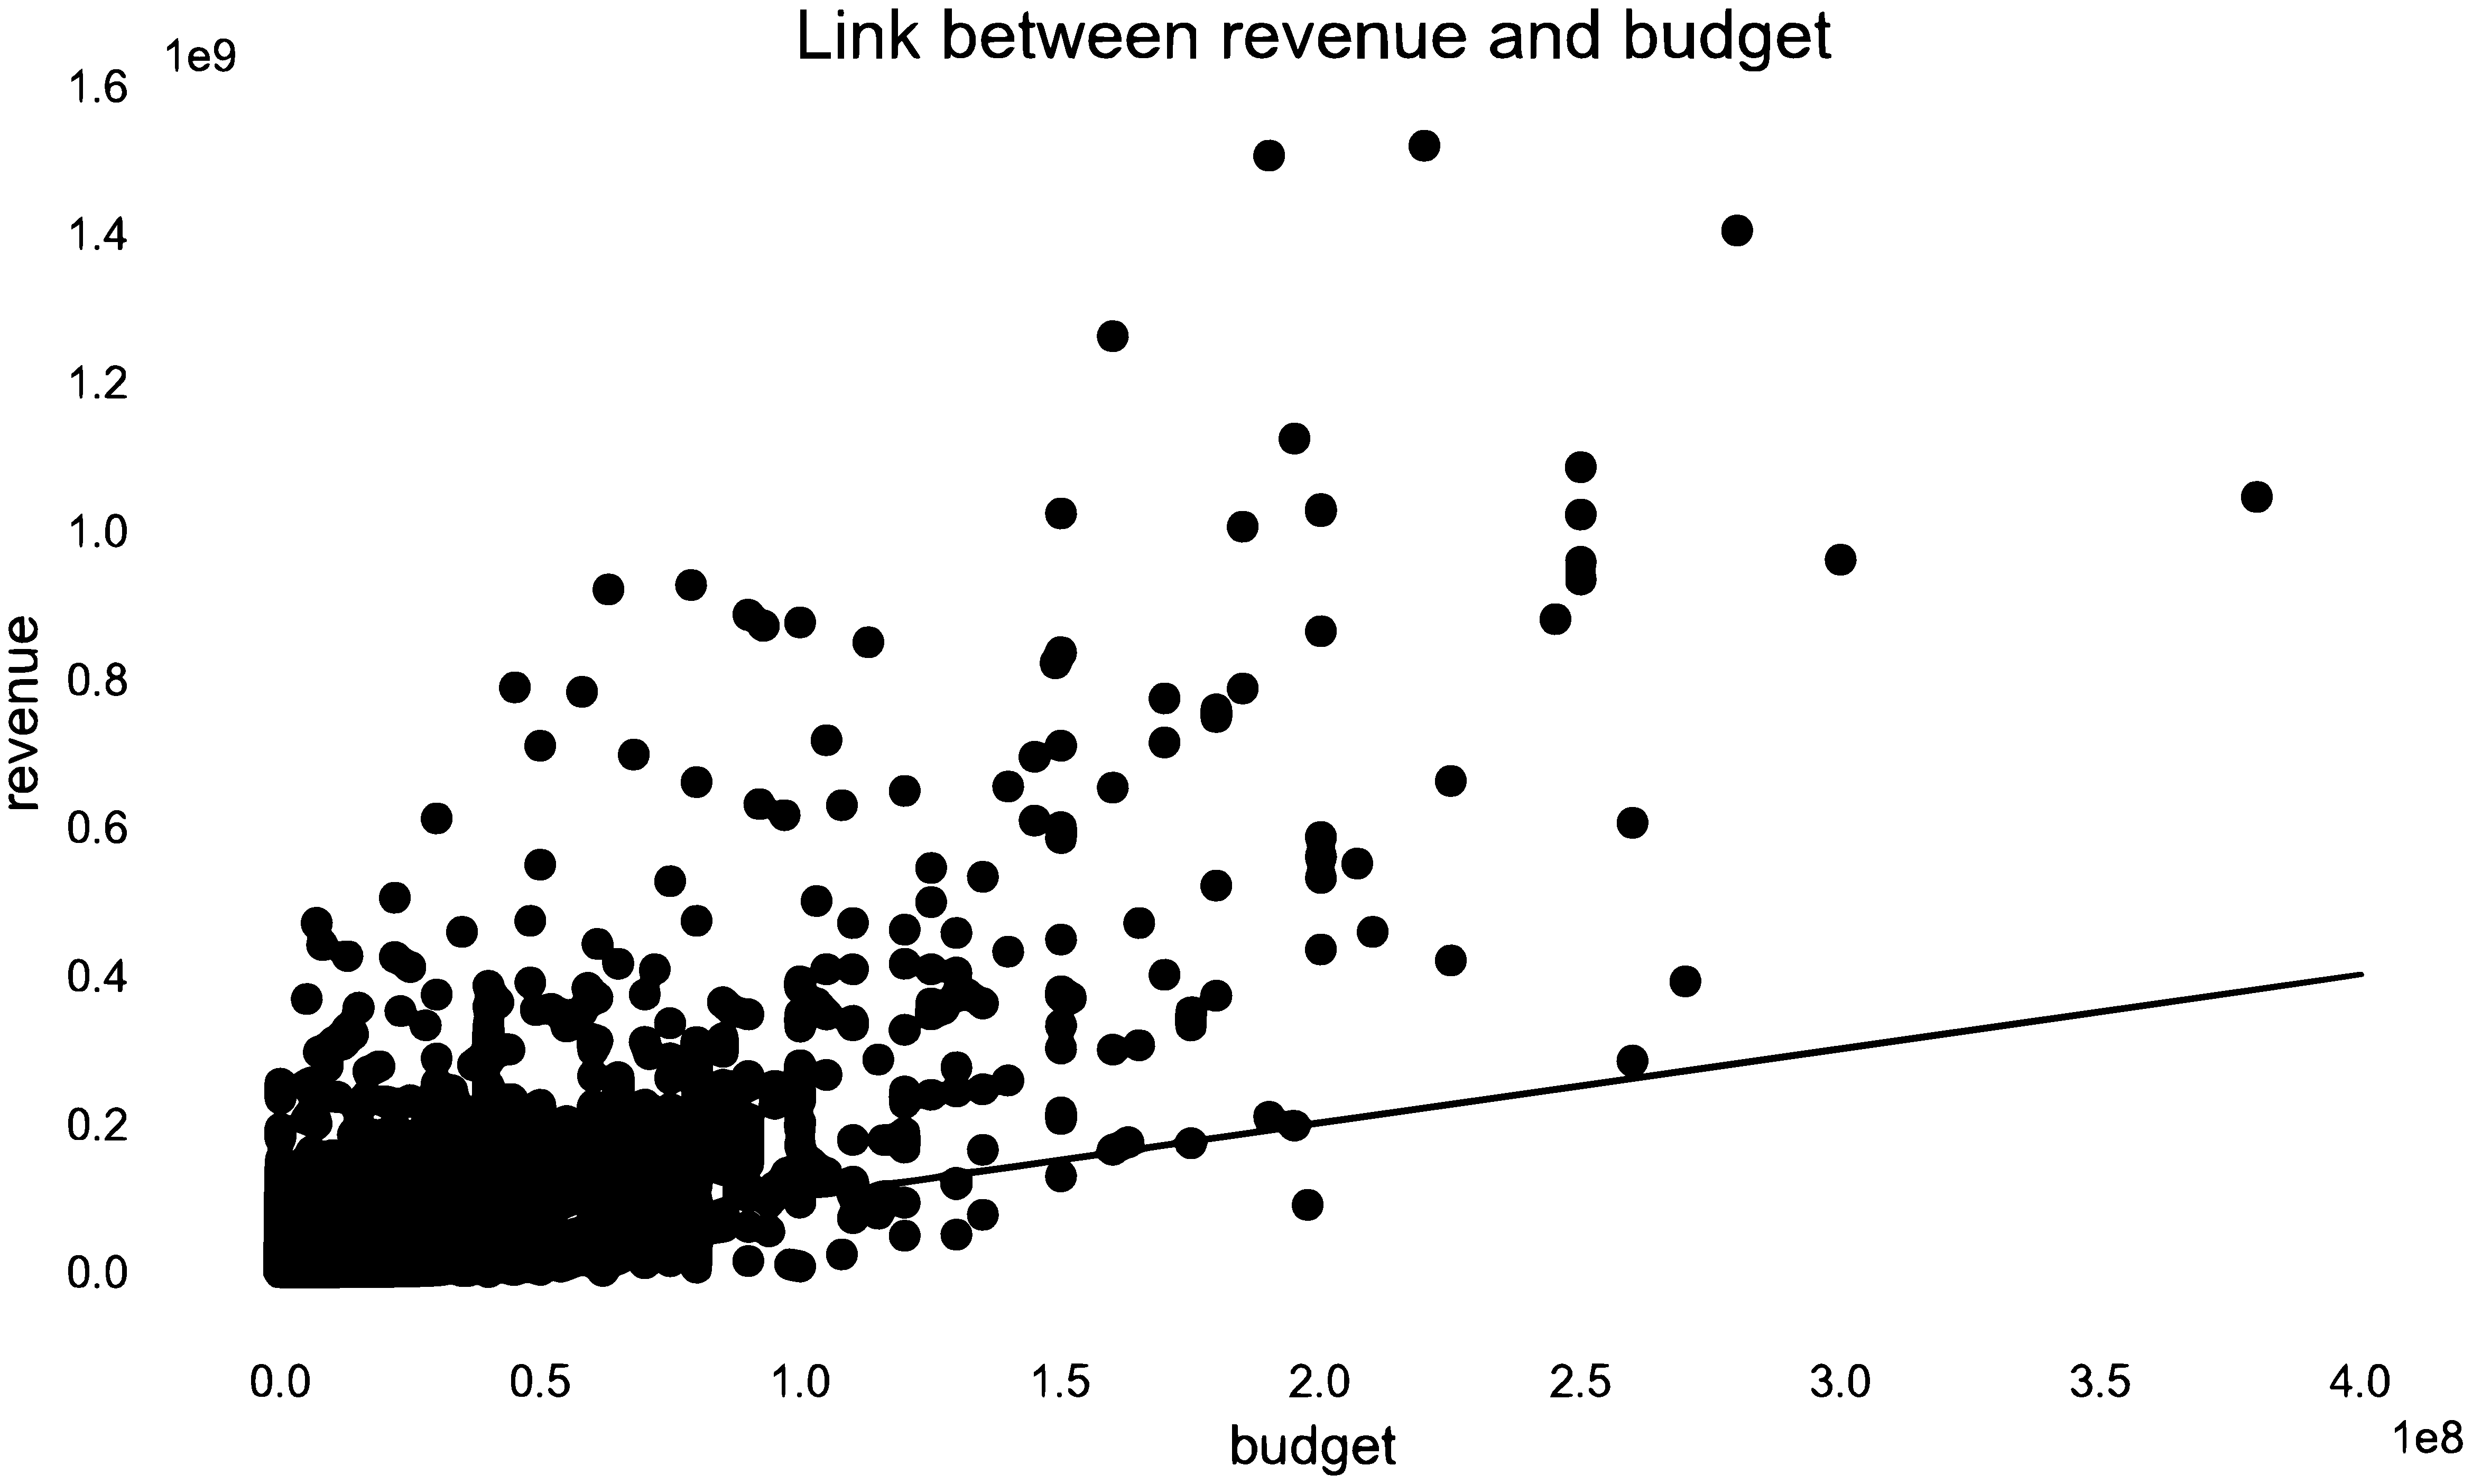
\includegraphics[scale=0.05]{logos/1.eps}
	\caption{Link between budget and revenue}%图片标题
	\end{figure}

   \begin{figure}[ht]%插入图片
   	\centering%用于居中
   	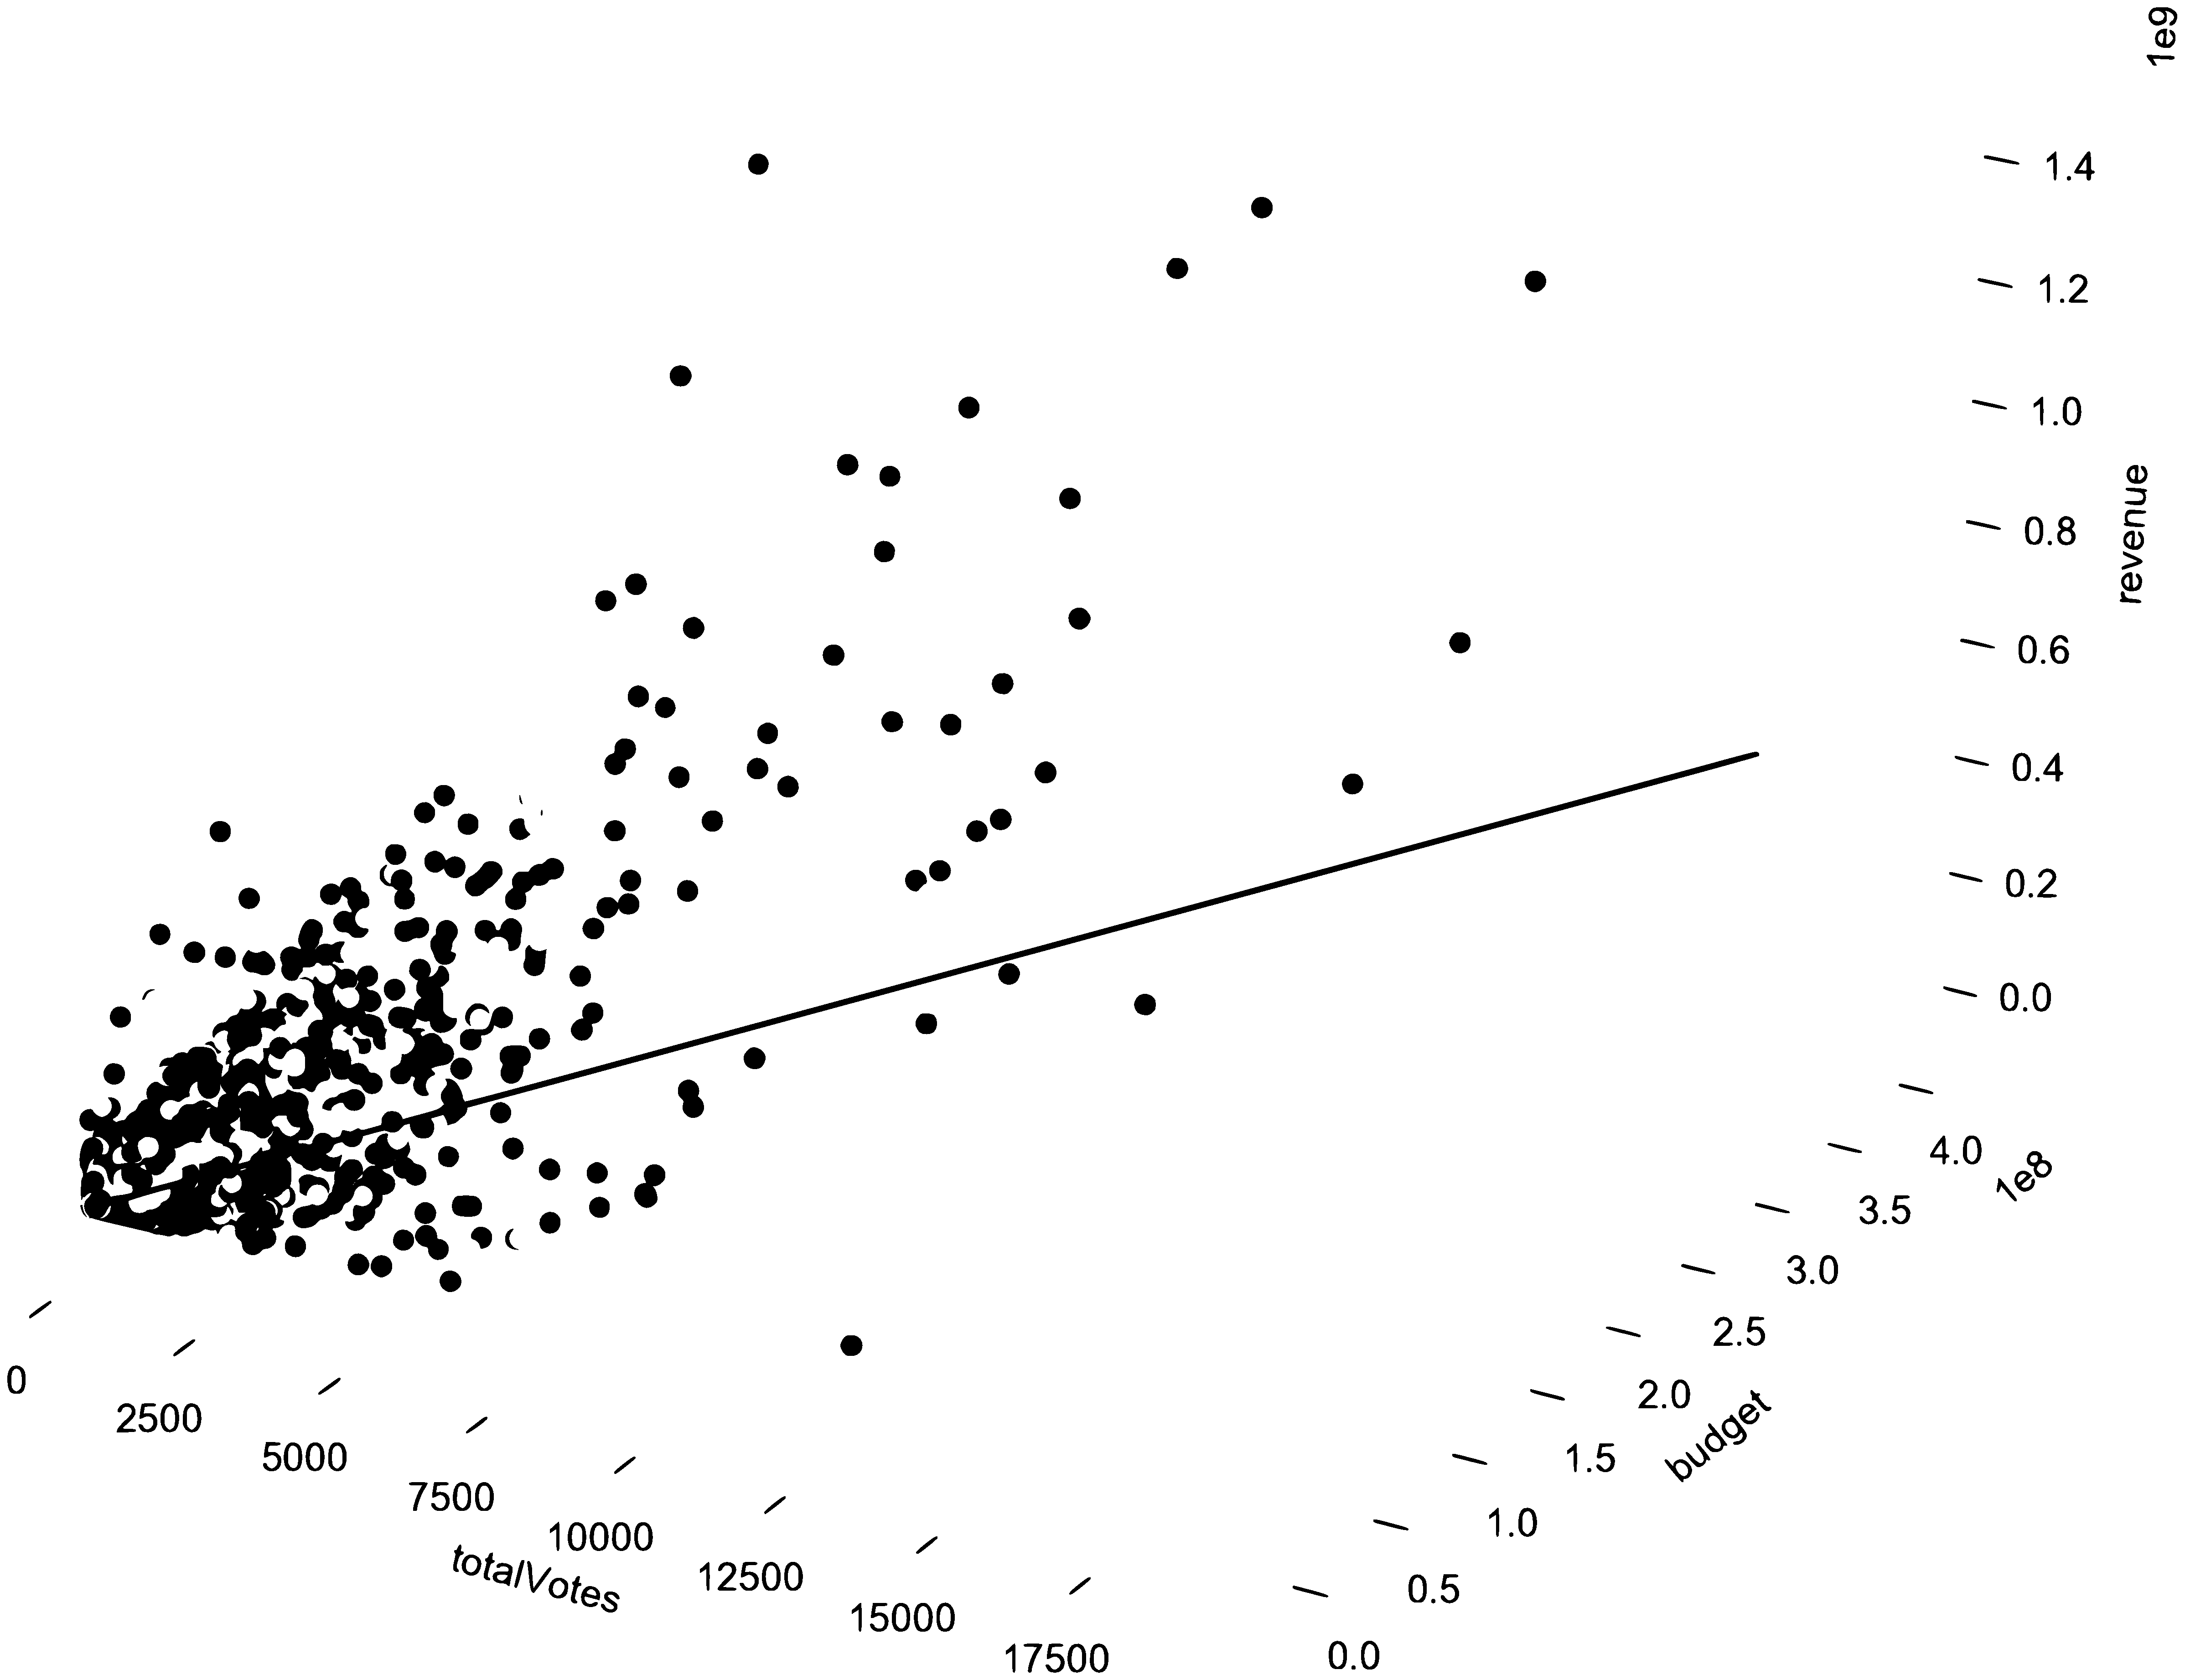
\includegraphics[scale=0.05]{logos/2.eps}
   	\caption{Link between budget and revenue and totalvotes}%图片标题
   \end{figure}

 As can be seen from the picture, the box office is not only related to the budget, but also related to the public evaluation

\end{slide}

\begin{slide}{ Data Visulization}
	
	\begin{figure}[ht]%插入图片
		\centering%用于居中
		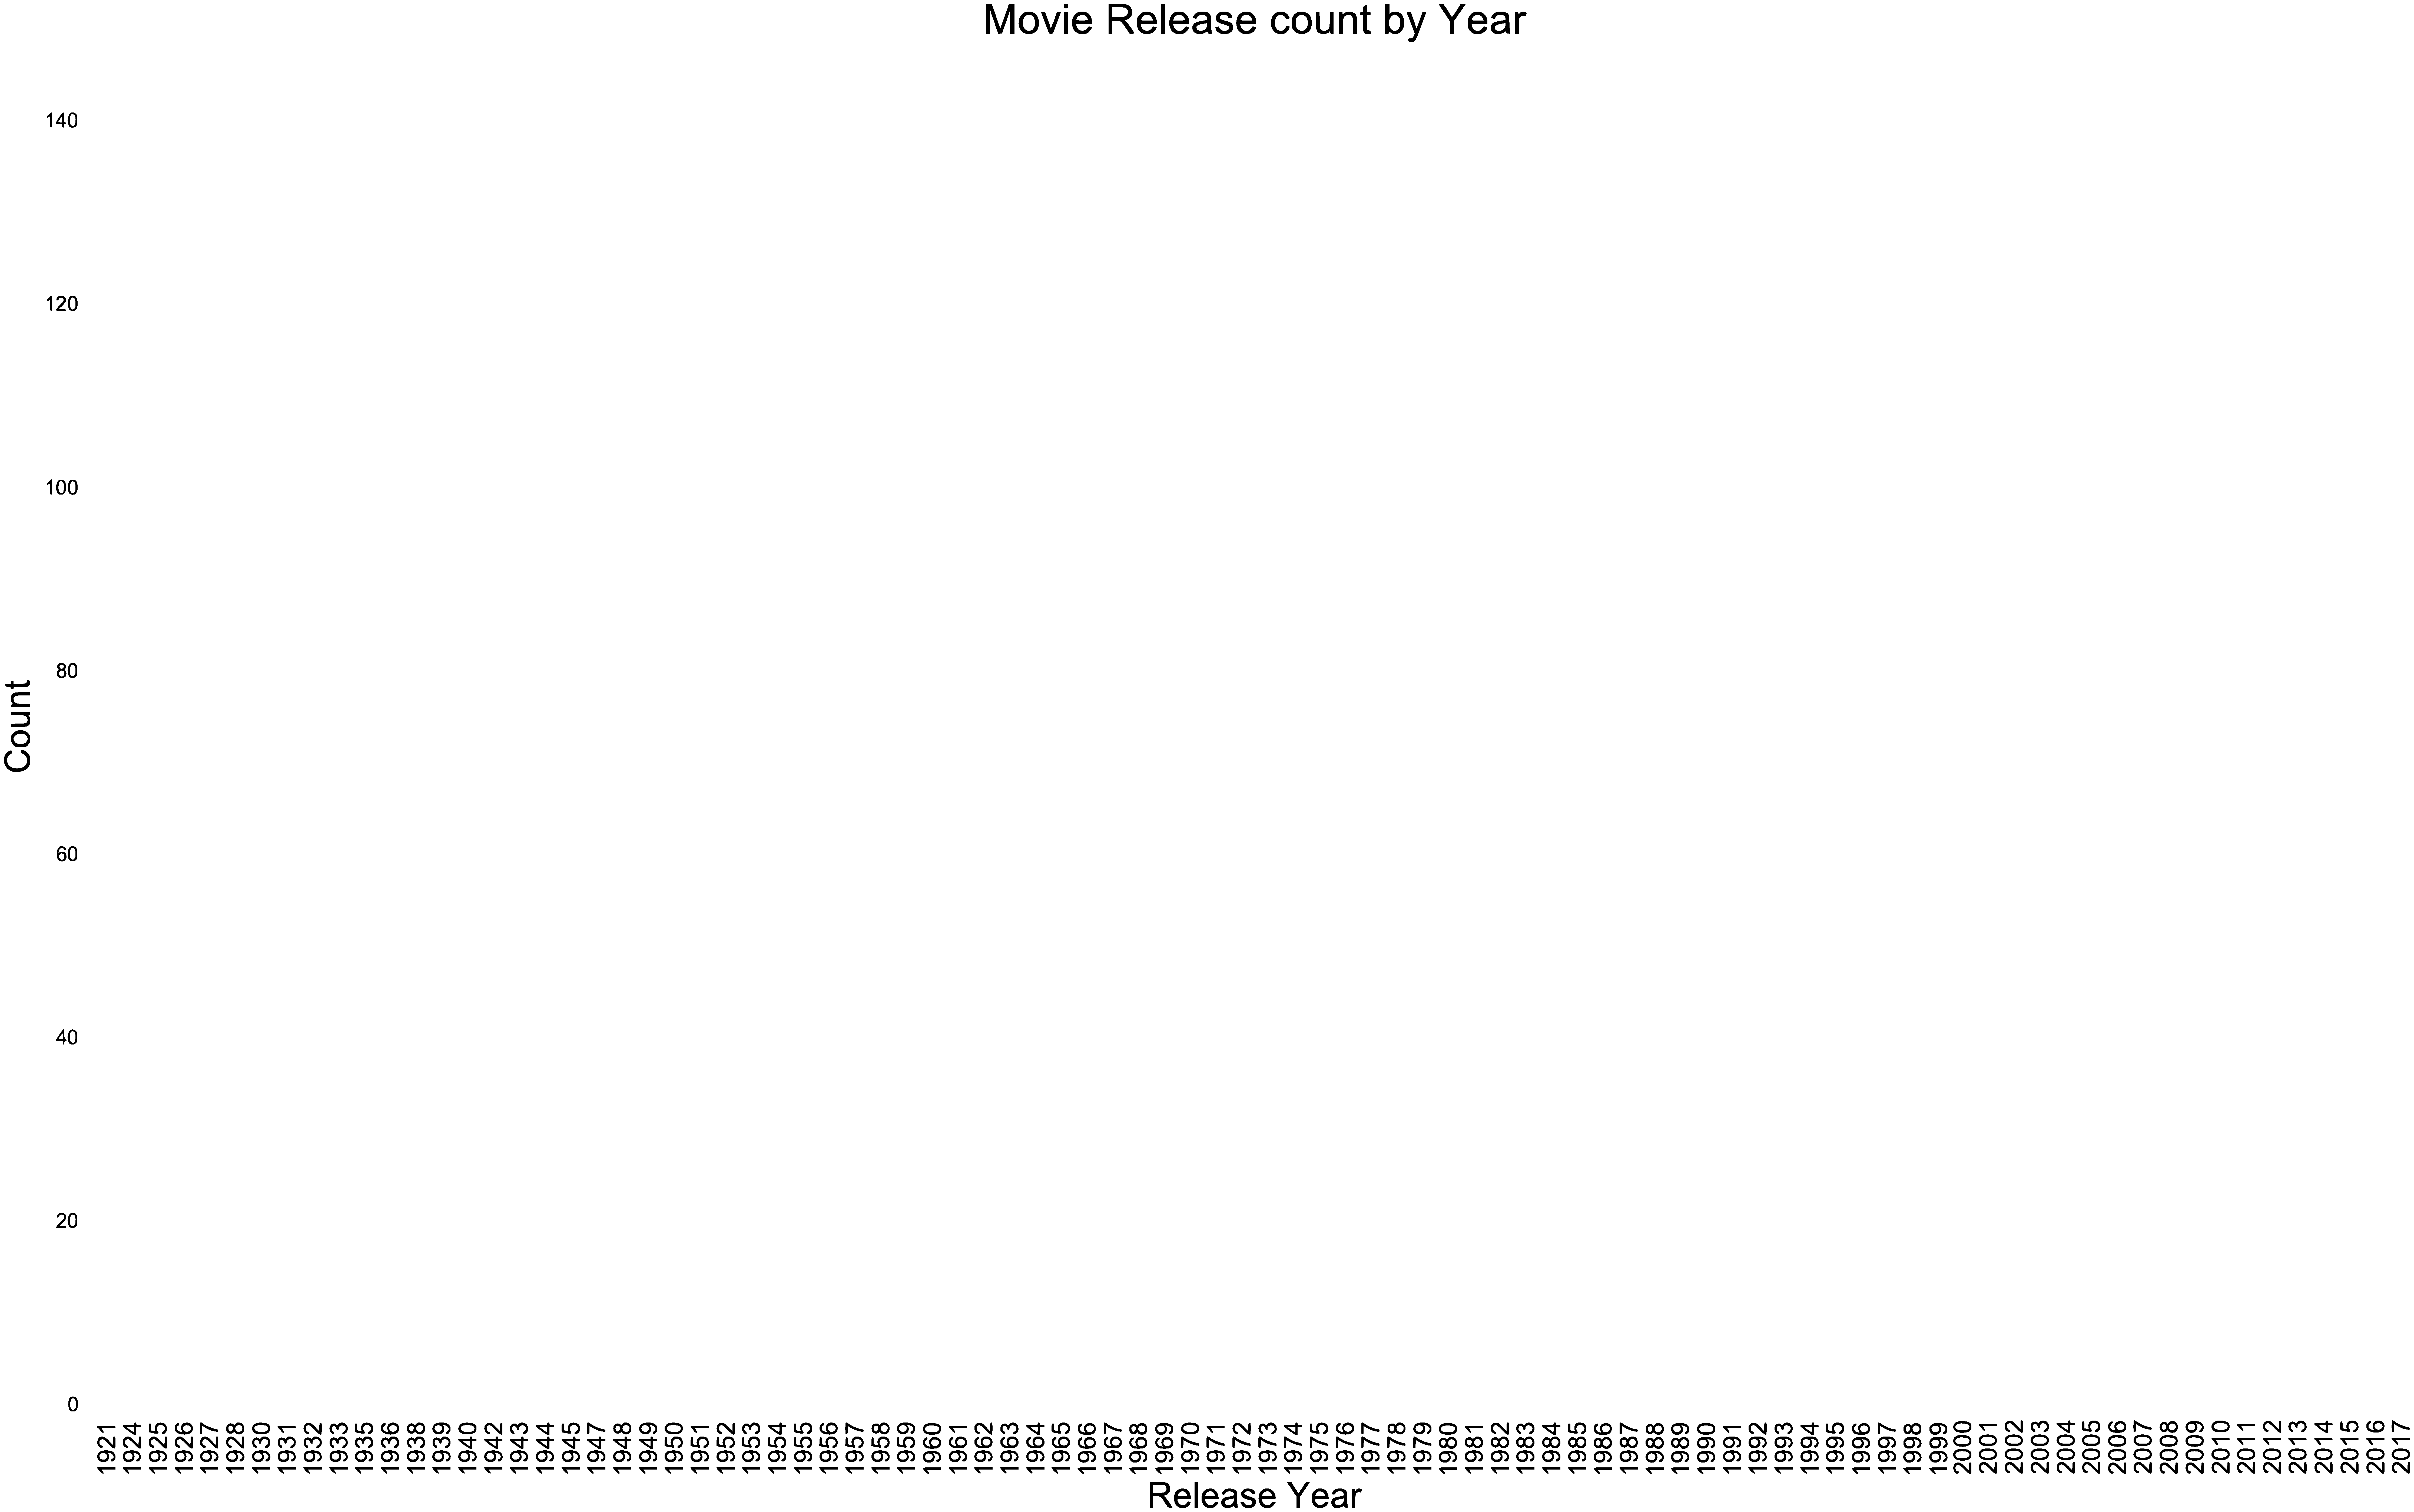
\includegraphics[scale=0.05]{logos/3.eps}
		\caption{Movie release count by year}%图片标题
	\end{figure}
	
	\begin{figure}[ht]%插入图片
		\centering%用于居中
		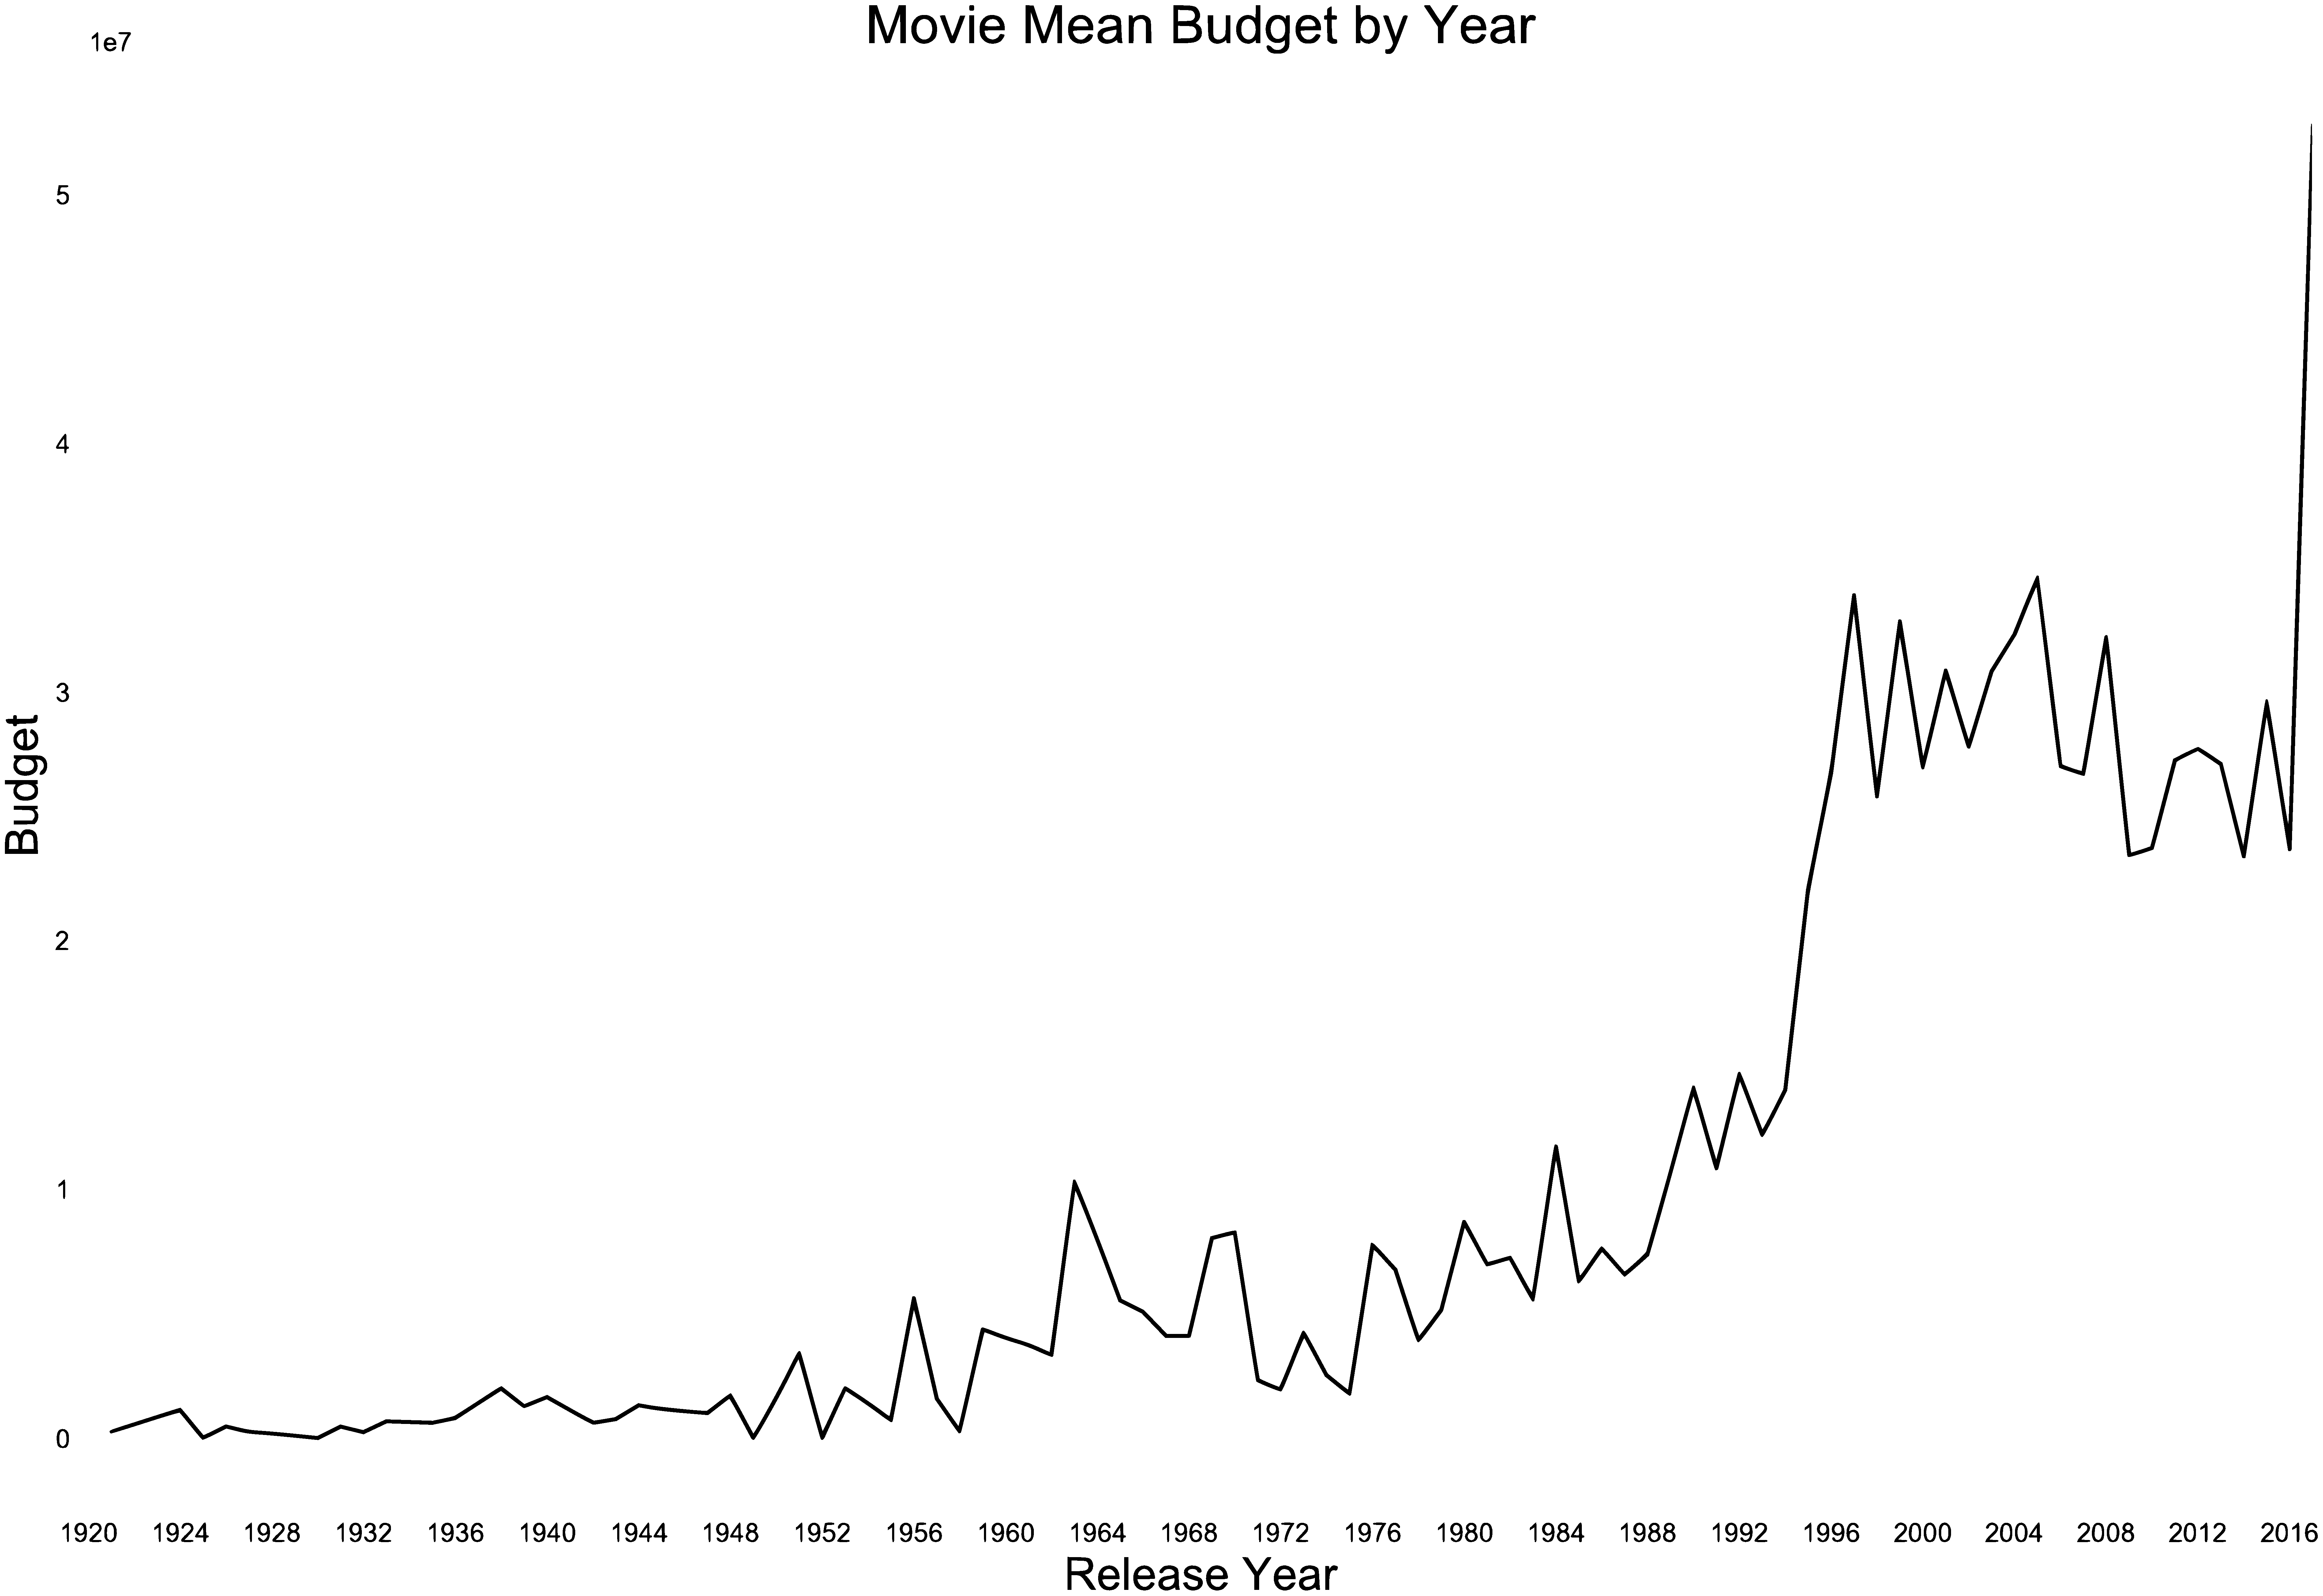
\includegraphics[scale=0.2]{logos/4.eps}
		\caption{Movie mean budget by year}%图片标题
	\end{figure}

    \begin{figure}[ht]%插入图片
	\centering%用于居中
	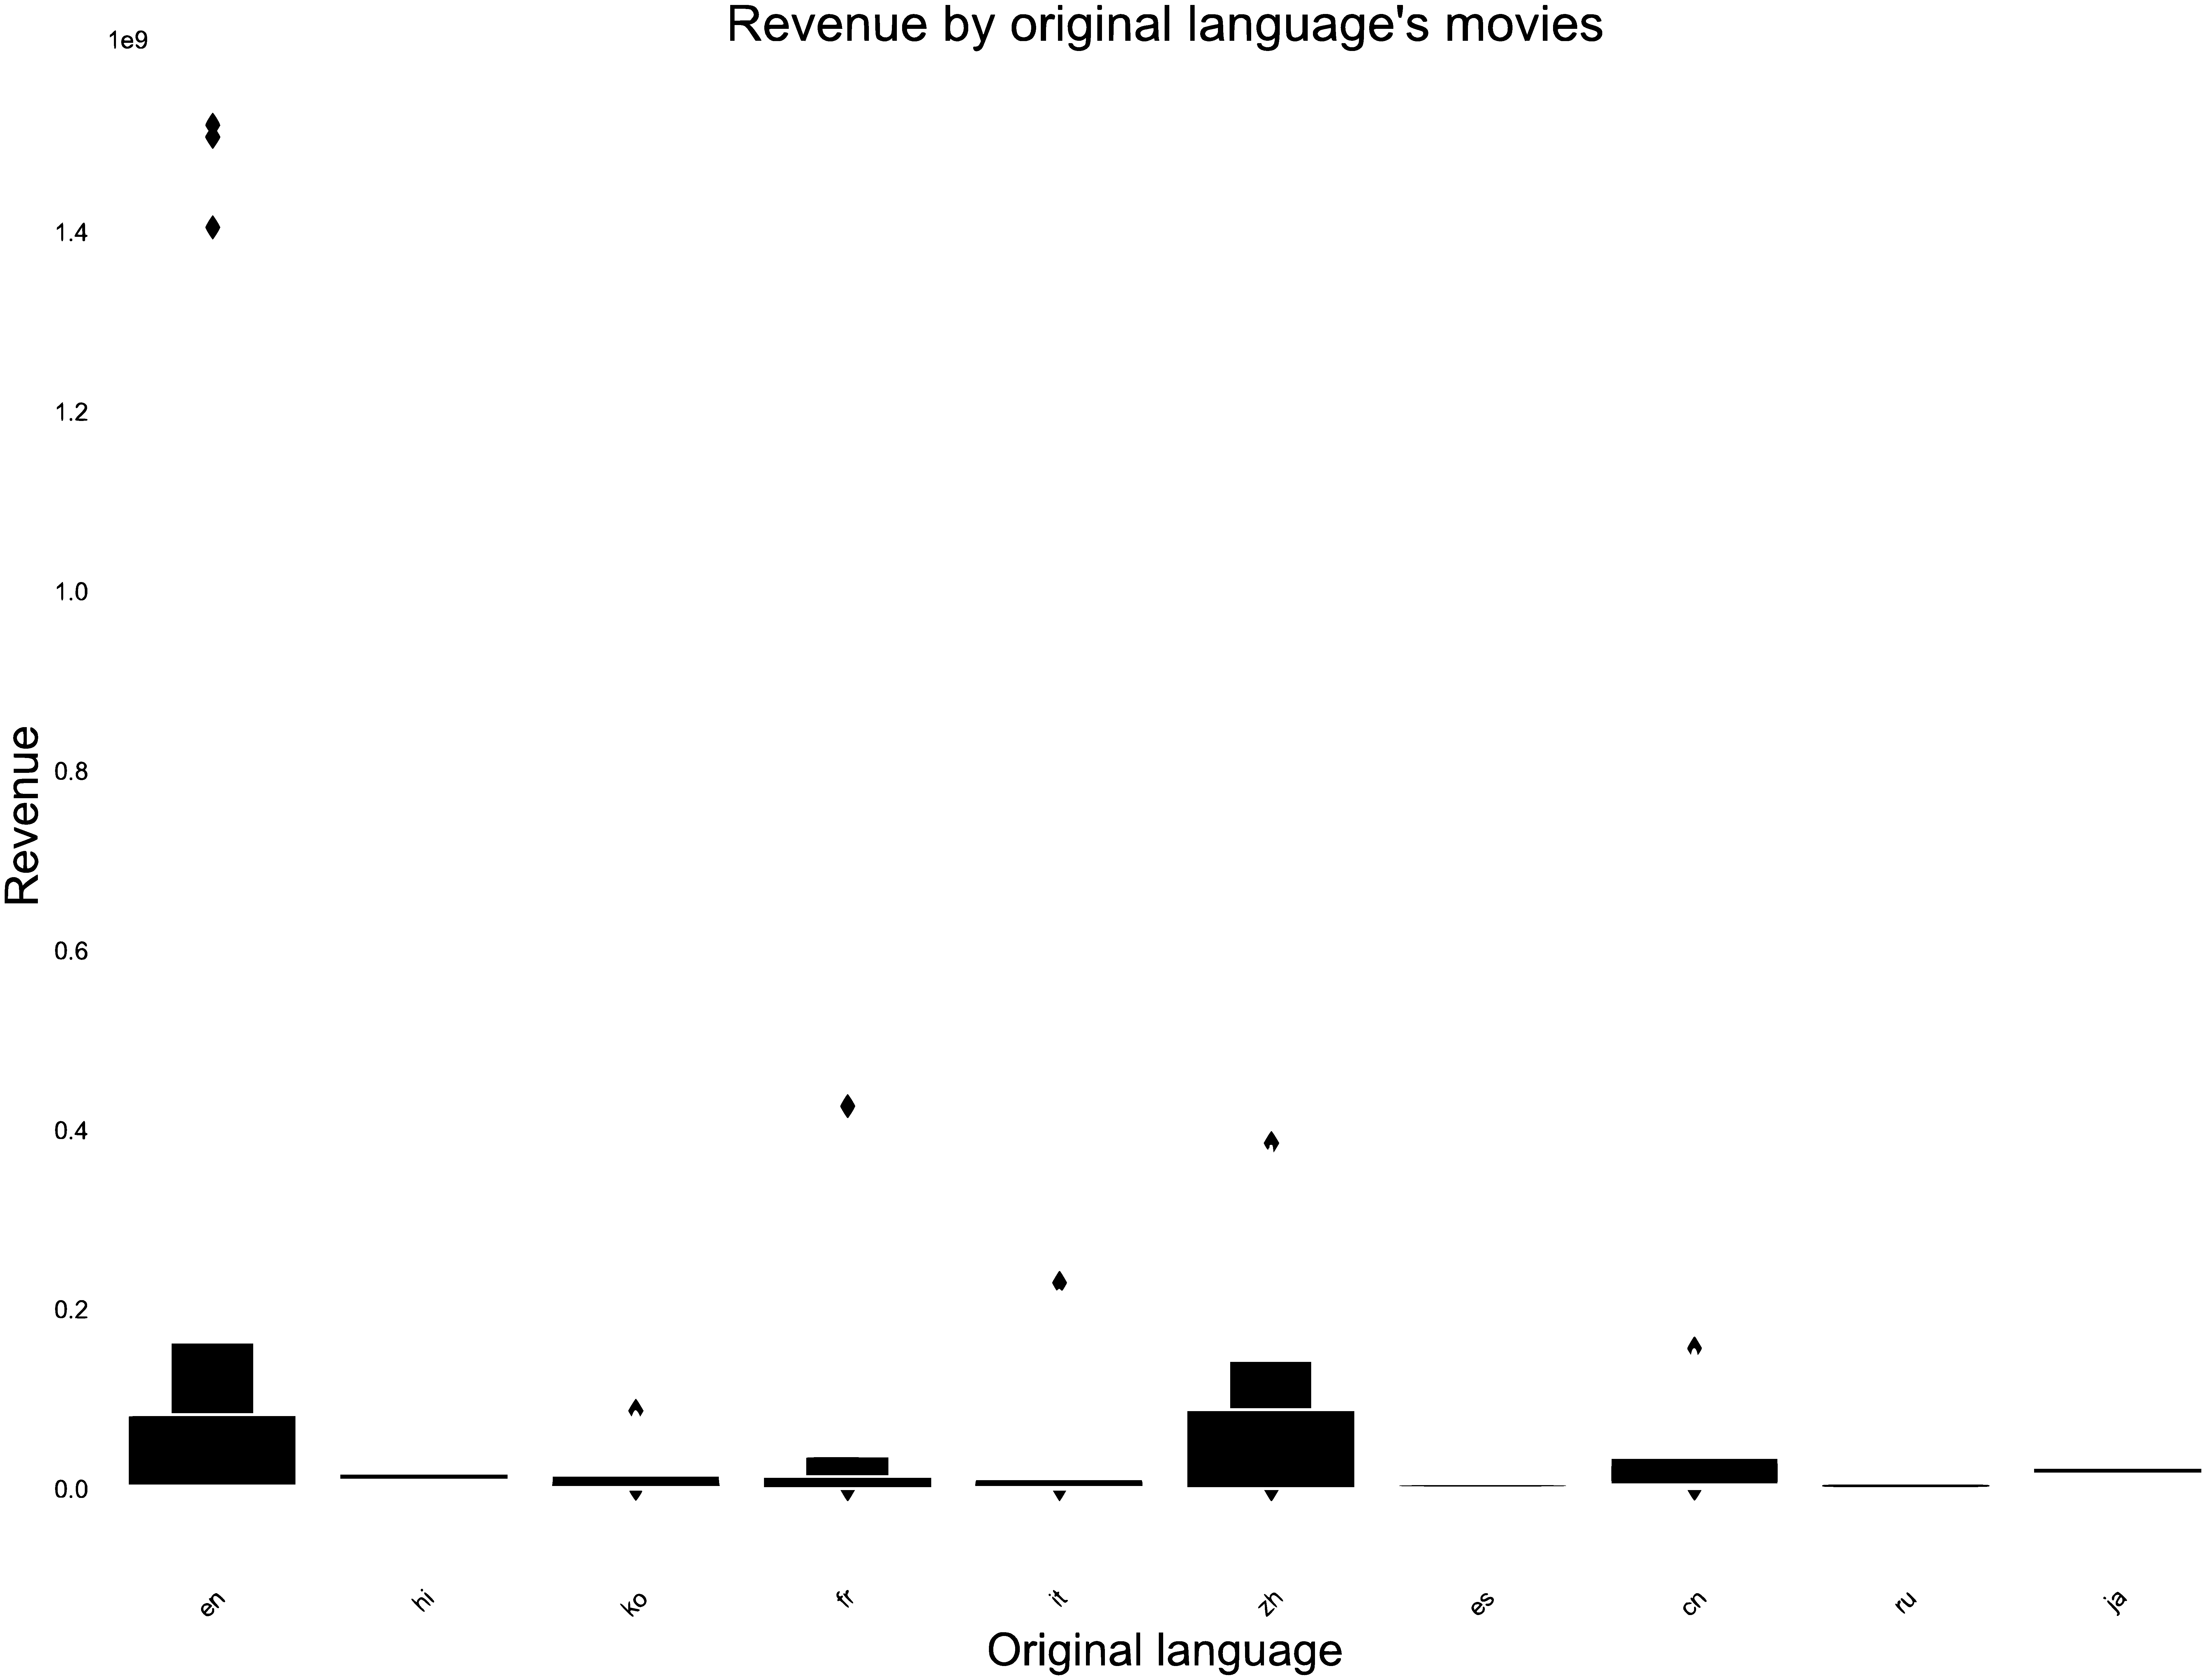
\includegraphics[scale=0.05]{logos/5.eps}
	\caption{Movie mean revenue by year}%图片标题
    \end{figure}

    \begin{figure}[ht]%插入图片
	\centering%用于居中
	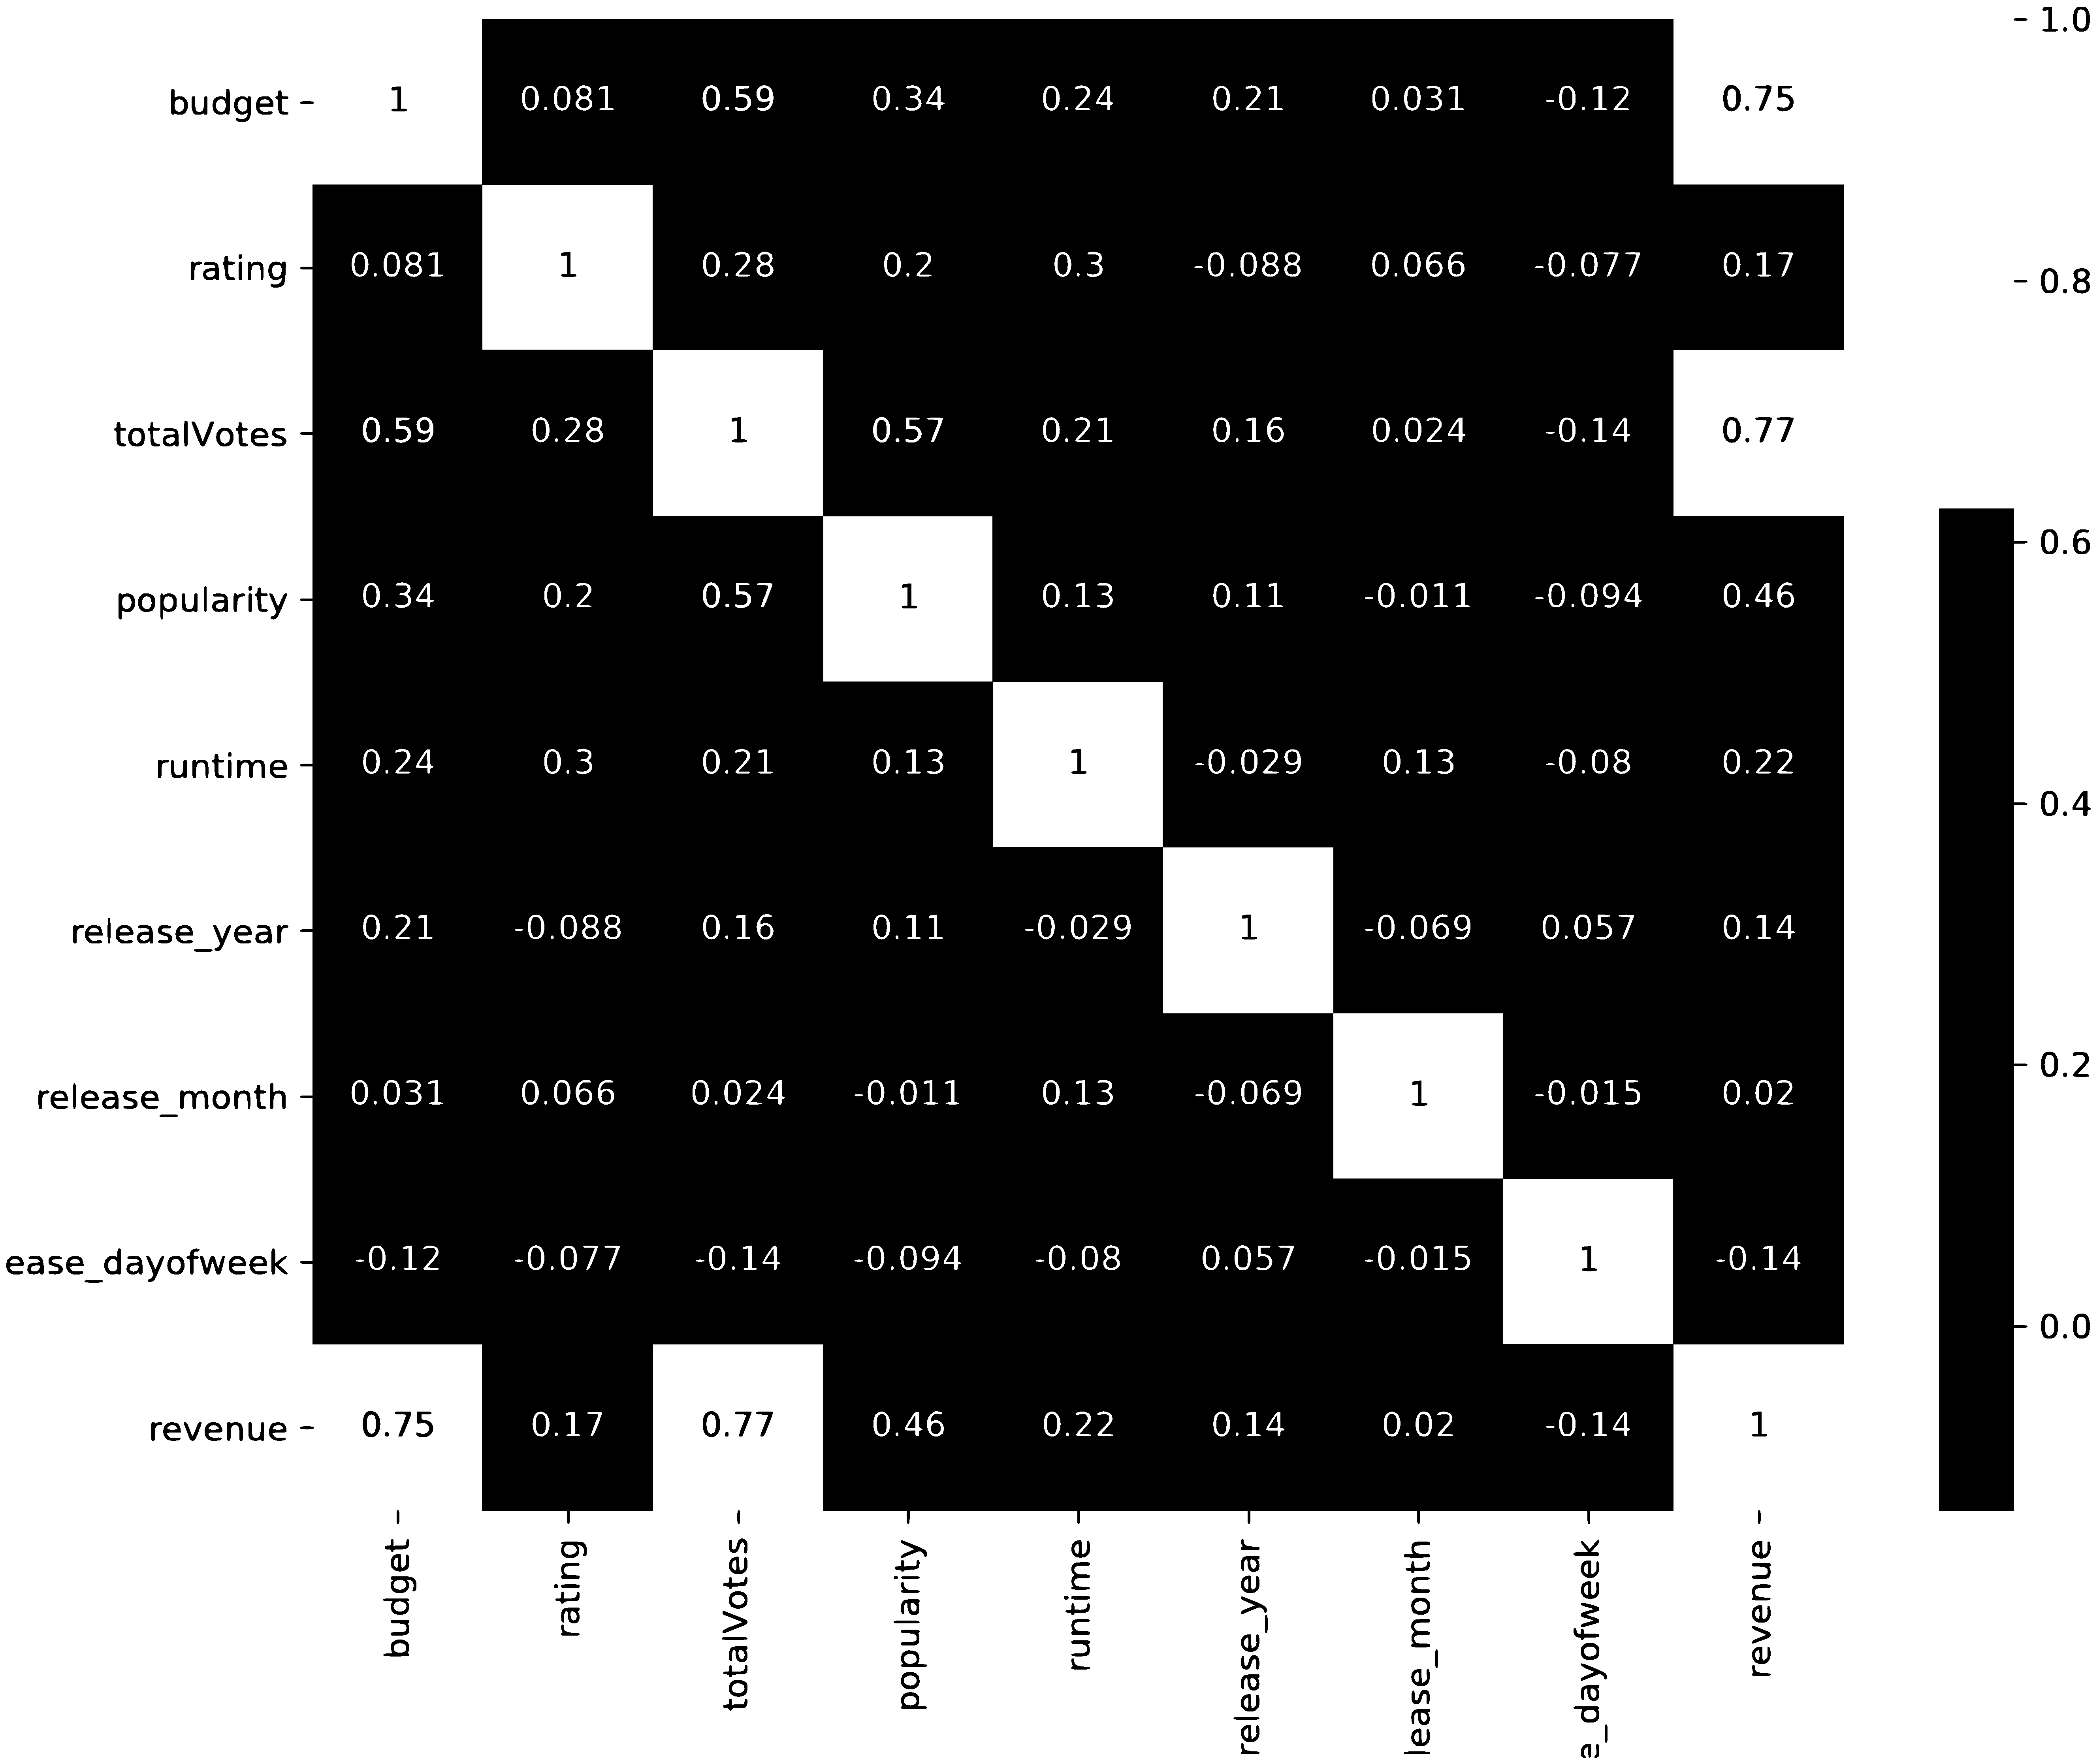
\includegraphics[scale=0.05]{logos/6.eps}
	\caption{Revenue by riginal language's movies}%图片标题
    \end{figure}
	
	%\vspace{0.5cm}	In recent years, both the investment and the box office of the film market have a relatively large growth, indicating that the film market is hot.It also reminds us that subsequent feature projects need to focus on the release year of the film.See the box office in the language of the film.En stands for English.After all, the world's languages, regardless of the size of the box office or the box office hot style, are the first.Zh is the one in your mind, Chinese.It can be seen that Chinese movies can surpass English.The language also reflects the box office.
	%\vspace{1cm}

	
\end{slide}

\begin{slide}{ Data Visulization}
	
	\begin{figure}[ht]%插入图片
		\centering%用于居中
		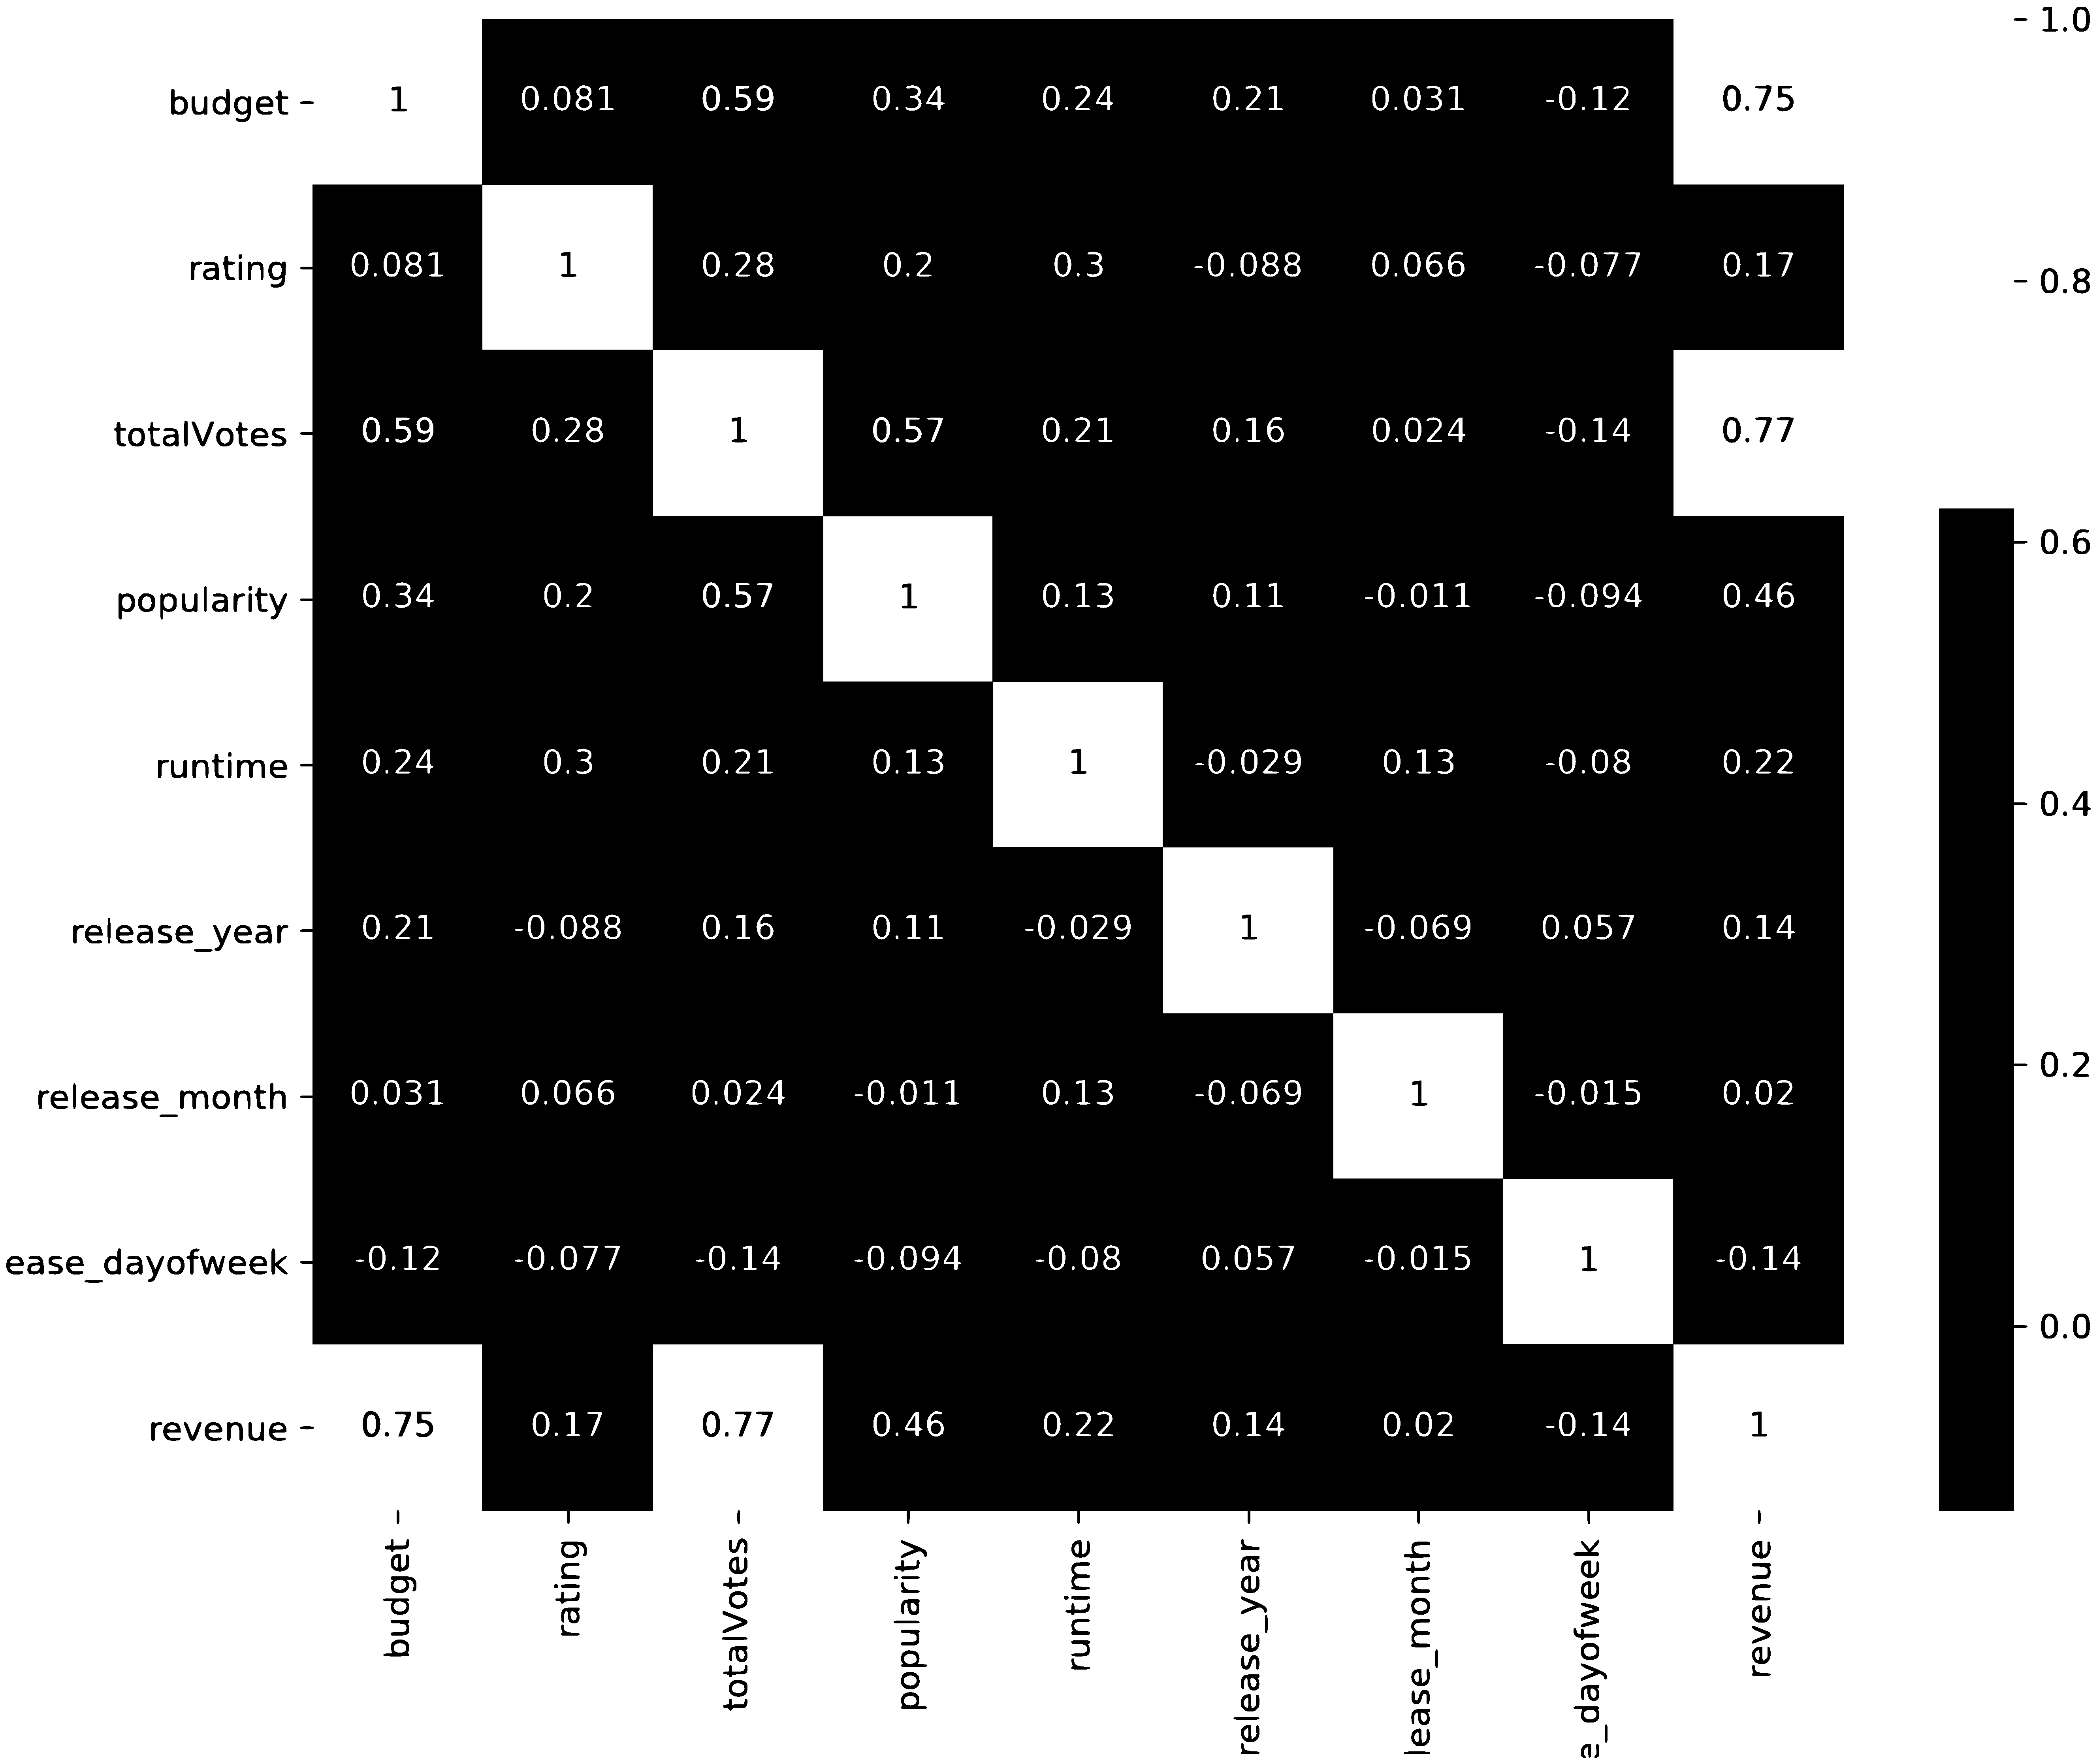
\includegraphics[scale=0.08]{logos/7.eps}
		\caption{Principal feature correlation}%图片标题
	\end{figure}
	
	\vspace{0.5cm}The Pearson coefficient (linear correlation coefficient) of the main features with the box office and the coefficients of each other are observed in the thermal diagram.It can be seen that budget, totalVotes and popularity are most related to the box office revenue
	\vspace{1cm}

	
\end{slide}

%\begin{slide}{Plot statistical charts and see the sale pattern} 
%By using the matplotlib to plot the photoes which describe the sale pattern
%\vspace{1cm}
%\begin{figure}[ht]%插入图片
  %\centering%用于居中
  %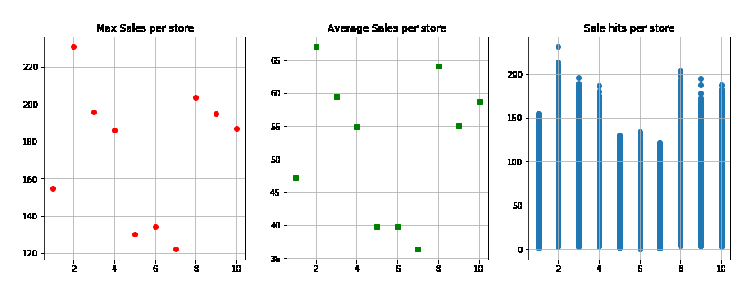
\includegraphics[scale=0.9]{E:/tulip-flip/templatex-master/powerdot-tuliplab/logos/0003.eps}
  %\caption{Displaying the sale pattern}%图片标题
  %\end{figure}
  %\vspace{0.5cm}
%From the figures we can know that 2nd store is the topper and 7th store is the least revenue generating one
%\end{slide}

%\begin{slide}{Variation in scale of the sale transacted}
%Displaying the distribution of sales volume 
%\vspace{1cm}
%\begin{figure}[ht]%插入图片
  %\centering%用于居中
  %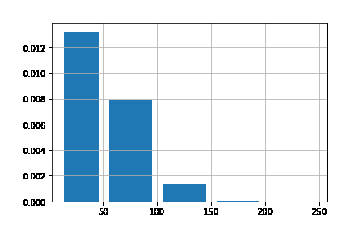
\includegraphics[scale=1.0]{E:/tulip-flip/templatex-master/powerdot-tuliplab/logos/0004.eps}
  %\caption{sales volume's distribution}%图片标题
  %\end{figure}
  %\vspace{1cm}
  %From this figure we can know that more and more sales volume is belong to [0,50]
%\end{slide}

%\begin{slide}{Store total sales}
%Displaying the total sales of the stores 
%\vspace{1.0cm}
%\begin{figure}[ht]%插入图片
  %\centering%用于居中
  %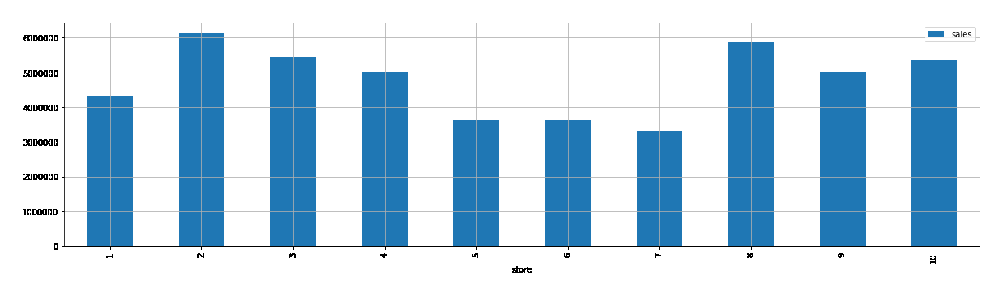
\includegraphics[scale=1.0]{E:/tulip-flip/templatex-master/powerdot-tuliplab/logos/0005.eps}
  %\caption{The total sales of all stores}%图片标题
  %\end{figure}
  %\vspace{0.5cm}
  %From this figure we can know that 2nd store is the topper of the all stores
%\end{slide}

%\begin{slide}{Item total sales}
  %Displaying the total sales of the items 
  %\vspace{0.8cm}
  %\begin{figure}[ht]%插入图片
    %\centering%用于居中
    %\includegraphics[scale=0.7]{E:/tulip-flip/templatex-master/powerdot-tuliplab/logos/0006.eps}
    %\caption{The total sales of all items}%图片标题
   % \end{figure}
    %\vspace{0.3cm}
   % From this figure we can know the total sales of all items.Obviously,we can know every item's sales
%\end{slide}

%\begin{slide}{All store's performance}
%Displaying the all store's performance over the time
%\vspace{1cm}
%\begin{figure}[ht]%插入图片
  %\centering%用于居中
  %\includegraphics[scale=0.7]{E:/tulip-flip/templatex-master/powerdot-tuliplab/logos/0007.eps}
  %\caption{The performance of all stores}%图片标题
  %\end{figure}
  %From this figure we can know every stores sales changing overtime
%\end{slide}

%\begin{slide}{All item's performance}
  %Displaying the all items' performance over the time
  %\vspace{1.2cm}
  %\begin{figure}[ht]%插入图片
    %\centering%用于居中
    %\includegraphics[scale=0.7]{E:/tulip-flip/templatex-master/powerdot-tuliplab/logos/0008.eps}
    %\caption{The performance of all stores items}%图片标题
    %\end{figure}
    %From this figure we can know every item sales changing overtime 
  %\end{slide}

%\begin{slide}{Individual pattern of store's and item's sale}
%Displaying the performance of the individual score and item
%\vspace{1cm}
%\begin{figure}[ht]%插入图片
  %\centering%用于居中
  %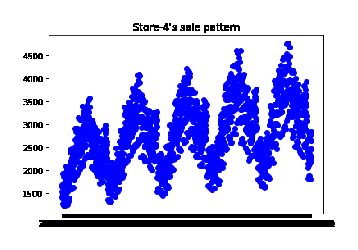
\includegraphics[scale=0.9]{E:/tulip-flip/templatex-master/powerdot-tuliplab/logos/0009.eps}
  %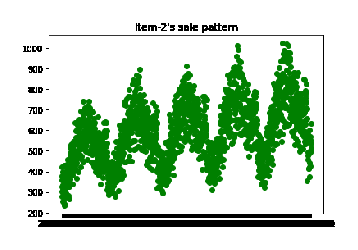
\includegraphics[scale=0.9]{E:/tulip-flip/templatex-master/powerdot-tuliplab/logos/0010.eps}
  %\caption{The performance of the individual store and item}%图片标题
  %\end{figure}
  %\vspace{0.8cm}
  %From this figure we can know individual pattern of item's sale and store's sale
%\end{slide}
\section{Modeling}

\begin{slide}[toc=,bm=]{Modeling}
\begin{itemize}
  \item Data exploration and feature engineering\\
\vspace{1cm}
  \item  Training data preparation
\vspace{1CM}
  \item  Model building, training, error testing
\end{itemize}
\end{slide}

\begin{slide}[toc=,bm=]{ Training results and errors}
\begin{itemize}
 
  \item DecisionTreeRegressor - RMSLE: 1.810177
  \item LinearRegression - RMSLE: 2.767681
  \item SVR - RMSLE: 1.720772
  \item KNeighborsRegressor - RMSLE: 1.616668
  \item RandomForestRegressor - RMSLE: 1.549074
  \item AdaBoostRegressor - RMSLE: 1.986040
  \item GradientBoostingRegressor - RMSLE: 2.011112
  \item BaggingRegressor - RMSLE: 1.531035
  \item ExtraTreeRegressor- RMSLE: 1.795049
  
  
\end{itemize}
\end{slide}

%\begin{slide}[toc=,bm=]{SVM}
 % \begin{itemize}
  %  \item Divide training data and test data
   % \item Do a model training
    %\item Model evaluation
    %\item Model prediction
  %\end{itemize}
%\end{slide}

%\begin{slide}[toc=,bm=]{The score of Random forest and SVM}
%  \begin{table}[htbp]  \centering
%   \caption{The score of 2 model}
%    \label{tbl:data information}
%    \begin{tabular}{ccccccc}
%      \hline
%      % after \\: \hline or \cline{col1-col2} \cline{col3-col4} %...
%       & model          & score \\
%      \hline
%      1 &  Random forest & 0.71  \\
%      2 &  SVM           & 0.79  \\
%      \hline 
%      %\bottomrule
%    \end{tabular}
%  \end{table}
%\end{slide}


%\begin{slide}[toc=,bm=]{Conclusion}
%  By using the above model, the prediction classification results can be obtained.\\ 
%\vspace{0.5cm}  The output is:\\
%\vspace{0.5cm} array(['southern_us', 'southern_us', 'italian', ..., 'italian',
%'southern_us', 'mexican'], dtype=object)
%\end{slide}

\section{Conclusion}

\begin{slide}[toc=,bm=]{Conclusion}
 In this period of study, I have been exposed to the relevant fields of feature engineering and data processing, and I just know some of them. There are still many pitfalls to tread in the learning process. In the next stage, I can learn more contents in data science and improve the quality of code.

\end{slide}
\section{Thanks}


%\begin{slide}[toc=,bm=]{}
  %\tableofcontents[content=sections]
  %\end{slide}
  %\section{Third section}
  %\begin{slide}[toc=,bm=]{Acknowledge}
  %\tableofcontents[content=currentsection,type=1]
  %\end{slide}
%\begin{slide}{Acknowledge}
%\vspace{3.5cm}
%\centering
%\huge
%\textit{Thank you for watching the slides} 
%\end{slide}
\end{document}

\endinput
